\documentclass[10pt]{article}
\usepackage{fullpage}
\addtolength{\textheight}{+40pt}
%% see: http://en.wikibooks.org/wiki/LaTeX/Page_Layout

\usepackage{authblk} %% author affiliation
%% see: https://tex.stackexchange.com/questions/214404/add-affiliations-to-the-authors-name-in-the-article-class 

\usepackage{graphicx}

\usepackage[T1]{fontenc}
\usepackage[latin1]{inputenc}

%%%%%%%%%%%%%%%%%%%%%%%%%%%%%%%%%%%%%%%%%%%%%%%%%%%%%%%%%%%%%%%%%%%%%
%% Place any additional packages needed here.  Only include packages
%% which are essential, to avoid problems later.
%%%%%%%%%%%%%%%%%%%%%%%%%%%%%%%%%%%%%%%%%%%%%%%%%%%%%%%%%%%%%%%%%%%%%
\usepackage{chemformula} % Formula subscripts using \ch{}

\usepackage{booktabs} %% professionally formatted tables

%% see: http://robjhyndman.com/researchtips/latex-floats/
\usepackage[section]{placeins}  %% change default float behaviour
\usepackage{afterpage}

\usepackage{graphicx}
% The amssymb package provides various useful mathematical symbols
\usepackage{amssymb,amsmath}
% \url command
\usepackage{url}

%% place figures side-by-side
\usepackage{subfig}
%% be able to remove subfigure captions (a), (b), etc.
\usepackage{caption}

%% better character output in PDFs
\usepackage{pslatex}

%% sideways table
\usepackage{rotating}

%% Allow suppression of caption labels aka Figure 1:
%% \usepackage{caption}

%% Caption modification ``Supplementary Table''
\renewcommand{\figurename}{Figure}
\renewcommand{\tablename}{Table}
\renewcommand{\listfigurename}{Supplementary Figures}
\renewcommand{\listtablename}{Supplementary Tables}

%%%%%%%%%%%%%%%%%%%%%%%%%%%%%%%%%%%%%%%%%%%%%%%%%%%%%%%%%%%%%%%%%%%%%
%% Place any additional macros here.  Please use \newcommand* where
%% possible, and avoid layout-changing macros (which are not used
%% when typesetting).
%%%%%%%%%%%%%%%%%%%%%%%%%%%%%%%%%%%%%%%%%%%%%%%%%%%%%%%%%%%%%%%%%%%%%

\newcommand{\todo}[1]{\rule{0.5em}{1ex}\hspace{0.3cm}\emph{to do:} #1\\}
% bold face around text with todo mark \todobf{text}
\newcommand{\todobf}[1]{{\rule{0.5em}{1ex}\textbf{ #1}}}

\newcommand{\C}{${}^\circ\mbox{C}$}
\newcommand{\degree}{~${}^\circ$}
\newcommand{\ul}{~$\mu$l}
\newcommand{\uM}{~$\mu$M}
\newcommand{\um}{~$\mu$m}
\newcommand{\ulmin}{~$\mathrm{\mu}$l/min}
\newcommand{\ugml}{~$\mathrm{\mu}$g/ml}
\newcommand{\ug}{~$\mathrm{\mu}$g}
\newcommand{\micro}{$\mathrm{\mu}$}
\newcommand{\A}{~{\AA}~}
\newcommand{\sd}{$\pm$}  %% +-

%%%%%%%%%%%%%%%%%%%%%%%%%%%%%%%%%%%%%%%%%%%%%%%%%%%%%%%%%%%%%%%%%%%%%
%% Title and Authors
%%%%%%%%%%%%%%%%%%%%%%%%%%%%%%%%%%%%%%%%%%%%%%%%%%%%%%%%%%%%%%%%%%%%%  
\begin{document}

\title{Supplemental Material:\\~\\
        From DNA on beads to proteins in a million droplets}

\author[1,2]{Ana Maria Restrepo Sierra}
\author[1]{Stefan Arold}
\author[1]{Raik Gr\"unberg}
\affil[1]
      {Department of Biological and Environmental Sciences and Engineering, King
        Abdullah University of Science and Technology, Thuwal, Saudi Arabia}
\affil[2]
      {present address: ...Delft...}

\date{}                %% remove date

\maketitle

\pagenumbering{gobble} %% switch off (rather than suppress) page numbering

\newpage
%%%%%%%%%%%%%%%%%%%%%%%%%%%%%%%%%%%%%%%%%%%%%%%%%%%%%%%%%%%%%%%%%%%%%
%% Table of Contents (TOC)
%%%%%%%%%%%%%%%%%%%%%%%%%%%%%%%%%%%%%%%%%%%%%%%%%%%%%%%%%%%%%%%%%%%%%
\tableofcontents
\listoffigures
\listoftables

\newpage
\pagenumbering{arabic}  %% switch page numbering back on

%% Counter modification ``S1, S2, ...''
\renewcommand{\thepage}{A\arabic{page}}
\renewcommand{\thetable}{S\arabic{table}}
\renewcommand{\thefigure}{S\arabic{figure}}

%%%%%%%%%%%%%%%%%%%%%%%%%%%%%%%%%%%%%%%%%%%%%%%%%%%%%%%%%%%%%%%%%%%%%
%% FIGURES
%%%%%%%%%%%%%%%%%%%%%%%%%%%%%%%%%%%%%%%%%%%%%%%%%%%%%%%%%%%%%%%%%%%%%
\section*{Supplemental Figures}
\vspace{4cm}


\begin{figure}[ht!] %% force float placement in current page
\begin{center}
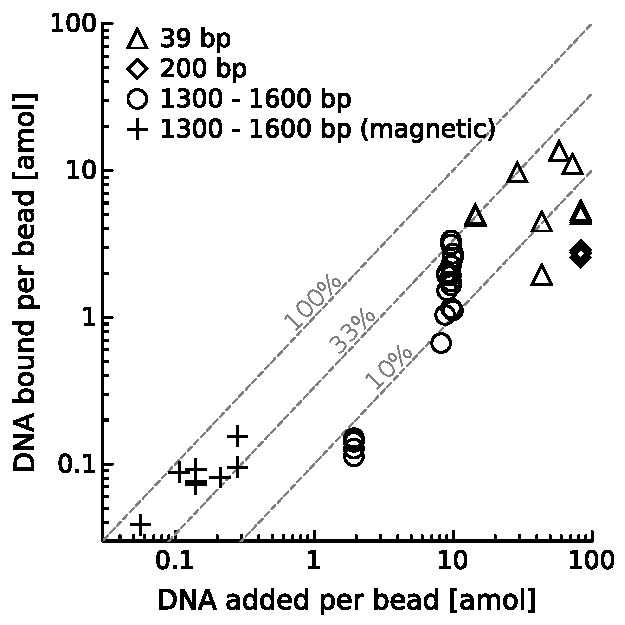
\includegraphics[width=0.6\textwidth]{figures/fig_dna.pdf}
\end{center} \label{sfig:single_concat}
\vspace*{-7mm} % space between labeling and the figure
\caption % This is what goes into Table of Content:
    [\label{sfig:bulkconcat} Expression from bound and unbound DNA fragments.]
    { % This is the text displayed below the figure:
      Comparison of cell-free expression levels from bound and unbound dsDNA.
    } 
\end{figure}

\afterpage{\clearpage}  %% force all floats to be placed
\newpage

%%%%%%%%%%%%%%%%%%%%%%%%%%%%%%%%%%%%%%%%%%%%%%%%%%%%%%%%%%%%%%%%%%%%%
%% TABLES
%%%%%%%%%%%%%%%%%%%%%%%%%%%%%%%%%%%%%%%%%%%%%%%%%%%%%%%%%%%%%%%%%%%%%
\section*{Supplemental Tables}
\vspace{2cm}

%% Constructs Table for supplement

\begin{table}[htp]

%%%%%%%%
%% Title
  \parbox{1.0\columnwidth}{\caption[Protein properties]{\label{stab:proteins}
      Proteins expressed in this study.}}

  \renewcommand{\arraystretch}{1.2}  %% increase line spacing

  \begin{tabular*}{1.0\columnwidth}{llccccc}

    %%%%%%%%%
    %% Header
    \toprule
    expressed from &
    composition &
    length &
    size &
    $\epsilon_{280}$ &
    $\lambda_{ex}$ &
    $\lambda_{em}$ 
    \\
    &
    &
    (aa) &
    (kD) &
    $(M cm)^{-1}$&
    (nm) &
    (nm)
    \\
    \midrule

    %%%%%%%
    %% Body

    me0052, rgf0049 & ALS-mScarletI-SpyTag-2Strep &
    449 & 49.0 & 60,850 & 569 & 593 \\

    rg3032, rgf0047 & FKBP-mNeon-WW-2Strep &
    447 & 48.9 & 77,810 & 506 & 517 \\

    sb0215, rgf0048 & 2Strep-LssmOrange-SpyTag &
    298 & 33.0 & 41,370 & 437 & 572 \\

    sb0201 & Bxb1-His$_{10}$ &
    515 & 58.1 & 86.400 & - & - \\


    %%%%%%%%%
    %% Footer
    \bottomrule 
    \bottomrule

  \end{tabular*}
\end{table}

 %% \label{stab:proteins}

%%%%%%%%%%%%%%%%%%%%%%%%%%%%%%%%%%%%%%%%%%%%%%%%%%%%%%%%%%%%%%%%%%%%%
%% The appropriate \bibliography command should be placed here.
%% Notice that the class file automatically sets \bibliographystyle
%% and also names the section correctly.
%%%%%%%%%%%%%%%%%%%%%%%%%%%%%%%%%%%%%%%%%%%%%%%%%%%%%%%%%%%%%%%%%%%%%
\bibliography{references}

\end{document}
